\documentclass[crop,tikz]{standalone}

\begin{document}
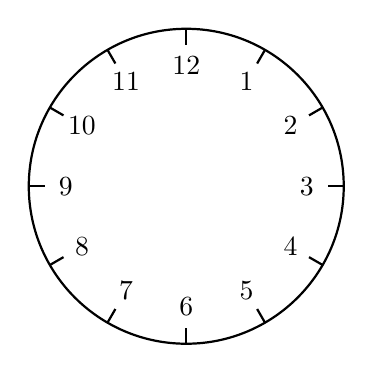
\begin{tikzpicture}[thick]
  \pgfmathsetmacro{\radius}{2}
  \pgfmathsetmacro{\markersize}{0.1*\radius}
  %
  \draw (0,0) circle (\radius);
  \foreach \num in {1,...,12} {
    \draw ({90-30*\num}:\radius) -- ({90-30*\num}:{\radius-\markersize});
    \node at ({90-30*\num}:{(\radius-\markersize)*0.85}) {\num};
  }
\end{tikzpicture}
\end{document}
